%%%%%%%%%%%%%%%%%%%%%%%%%%%%%%%%%%%%%%%%%%%%%%%%%%%%%%%%%%%%%%%%%%%%%%%%%%%%%%

\documentclass{l3deliverable}

%%%%%%%%%%%%%%%%%%%%%%%%%%%%%%%%%%%%%%%%%%%%%%%%%%%%%%%%%%%%%%%%%%%%%%%%%%%%%%

\usepackage{graphicx}%
%


\version{3.0}


\usepackage{tabularx}%
\usepackage{url}%
\usepackage{usecasedescription}%

%%%%%%%%%%%%%%%%%%%%%%%%%%%%%%%%%%%%%%%%%%%%%%%%%%%%%%%%%%%%%%%%%%%%%%%%%%%%%%
%% Check these macro values for appropriateness for your own document.

\title{Requirements Document}

\author{Michael Kilian\\
	Dan Tomosoiu\\
	Tony Lau\\
	Peeranat Fupongsiripan\\
	Hector Grebbel
}

\date{12 November 2012}

\deliverableID{D3}
\project{PSD3 Group Exercise 1}
\team{L}

%%%%%%%%%%%%%%%%%%%%%%%%%%%%%%%%%%%%%%%%%%%%%%%%%%%%%%%%%%%%%%%%%%%%%%%%%%%%%%

\begin{document}

%%%%%%%%%%%%%%%%%%%%%%%%%%%%%%%%%%%%%%%%%%%%%%%%%%%%%%%%%%%%%%%%%%%%%%%%%%%%%%

\maketitle

\tableofcontents

\newpage

%%%%%%%%%%%%%%%%%%%%%%%%%%%%%%%%%%%%%%%%%%%%%%%%%%%%%%%%%%%%%%%%%%%%%%%%%%%%%%
%% Standard section for all documents

\section{Introduction}
Software Engineering (SE) and Electronic and Software Engineering (ESE) students in the School
of Computing Science are required to complete an internship as part of their course, in the summer
between level 3 and level 4. An internship is a short period of time that a student spends working
within in a company in order to gain experience (from as little as a month up to a year). Internships
in the software industry are normally paid, although the rate offered can vary from company to
company. The School imposes requirements on these internships to ensure that the student receives
an appropriate experience for their degree programme. More details of these restrictions can be found
on the Software Engineering Summer Placement (SESP) moodle page.\\
\\
Currently, available internships are advertised to students on an ad-hoc basis through the SESP
moodle page. An organisation wishing to recruit an intern submits an advertisement to the course
coordinator, who publishes it on the course mailing list. The format and content of the advert can
vary widely, including information about the nature of the internship (what the successful applicant
will do), duration, expected start date, compensation, person requirements and so on. The course
coordinator checks each advert and comments on whether it is suitable for SE/ESE students, as students 
who are not enrolled on the SE/ESE scheme may also view the advertisements posted on
the SESP moodle page in order to obtain information about possible internships.\\
\\
Sometimes internships applications are managed through the Careers Service's Club21 website;
sometimes through the e-Placements scheme; and sometimes the company has its own system of
collecting applications. In addition, some advertisements are posted by academics in the school for
students to work with them during the summer vacation.\\
\\
The allocation of SE/ESE students to internships is tracked by the course coordinator separately,
using a Microsoft Access Database. Students are required to inform the coordinator when they have
secured a placement, which may or may not have been advertised on the SESP page. The coordinator
must then approve the internship if it is suitable for the student's course.\\
\\
The SESP course coordinator has decided that a unified system is necessary for collecting and
publishing internship advertisements, and for tracking which SE/ESE students have been successful
in securing them. An initial requirements analysis has found that the following features must be
supported by the system:
\begin{itemize}
\item{Submission of internship advertisements}
\item{Review, comment and publication of internship advertisements by the course coordinator}
\item{Review of advertisements by students}
\item{Notification of successful selection for an internship by an SE/ESE student}
\end{itemize}


\subsection{Related Documentation}
These documents are available in our team repository:
\begin{itemize}
	\item{Client interview questions}
	\item{Raw requirements list}
	\item{Interview audio recording}
	\item{Client consent form}
\end{itemize}

\subsection{Purpose and Description of Document}
This document displays the use cases we have identified for the system. The long term aim of the document is to add to it as new requirements are identified and to use it as a basis for system design. 

\subsection{Document Status and Schedule}
Naturally this document is under constant revision as new requirements are identified and as stakeholder conflicts are resolved\\
\\
This document should be revised weekly in time for the next PSD team meeting (Tuesday 11am), assuming any changes are required. A change log for this document is visible in the Appendix. Further information about changes can be viewed using githubs version tracking features.

%%%%%%%%%%%%%%%%%%%%%%%%%%%%%%%%%%%%%%%%%%%%%%%%%%%%%%%%%%%%%%%%%%%%%%%%%%%%%%

\newpage
\section{System Scope}
As specified in the initial business case, the system is only to be used within the Department of Computing Science. The only outside interaction comes from companies whosubmit advertisements to the system. \\
The process of a student applying for a placement is the most complex with regards to scope. In many cases larger companies will have their own websites or online applicationprocesses which they will wish the student to take part in. In this case the student does not apply through the system and will apply by using the details found in the correspondingadvert for the placement. However smaller, independant companies may not have their own process. For such companies the system will handle direct applications by the student to the company. Finally the student may also find placements entirely on their own. When this occurs the student should submit information about the placement through the system, butthe application to the placement is outside the system scope.\\

%%%%%%%%%%%%%%%%%%%%%%%%%%%%%%%%%%%%%%%%%%%%%%%%%%%%%%%%%%%%%%%%%%%%%%%%%%%%%%

\subsection{System Actors}
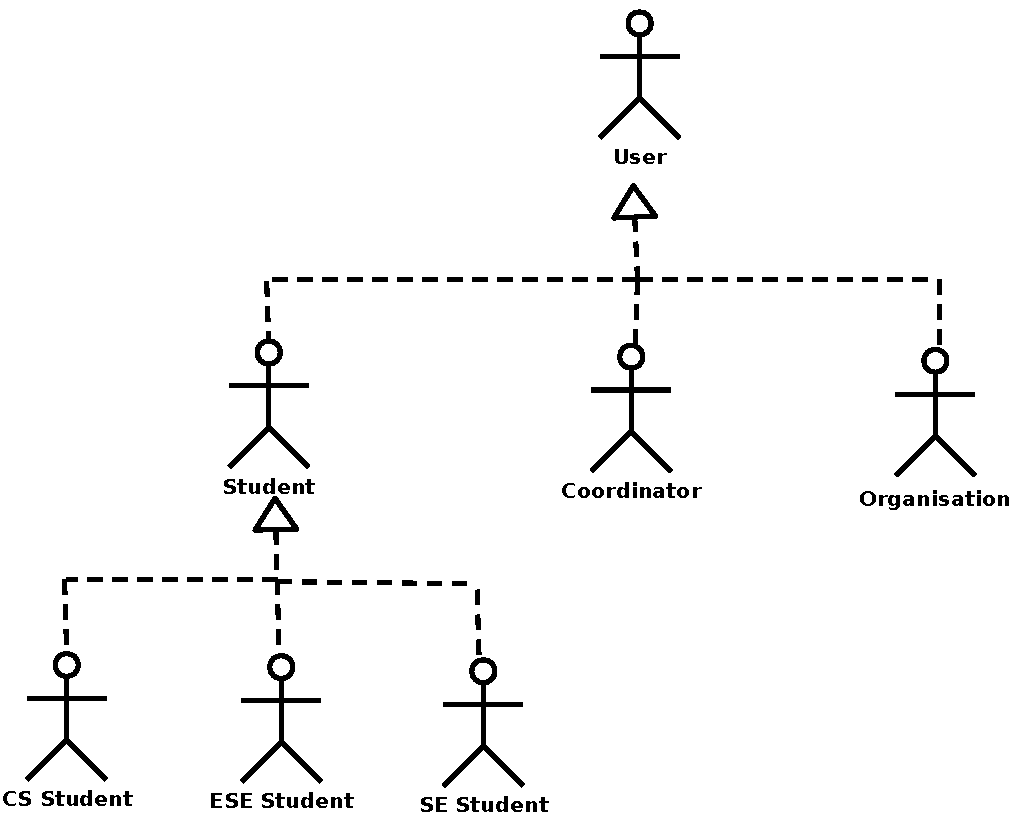
\includegraphics[scale = 0.5]{Actors.pdf}

The above diagram shows the actor roles present in the system:
\begin{itemize}
\item{\textbf{Student:}\ all students enrolled in the system who can apply for placements. This can be further broken down into CS, SE and ESE students, who will have
different rules on what constitues a suitable placment.}
\item{\textbf{Coordinator: }\ the course coordinator will have privileges to approve and reject files, view student progress, etc.}
\item{\textbf{Organisation: }\ any group who advertises placements to the system. This may include external companies, intership schemes and university groups.}
\end{itemize}
%%%%%%%%%%%%%%%%%%%%%%%%%%%%%%%%%%%%%%%%%%%%%%%%%%%%%%%%%%%%%%%%%%%%%%%%%%%%%%

\subsection{Domain Model}
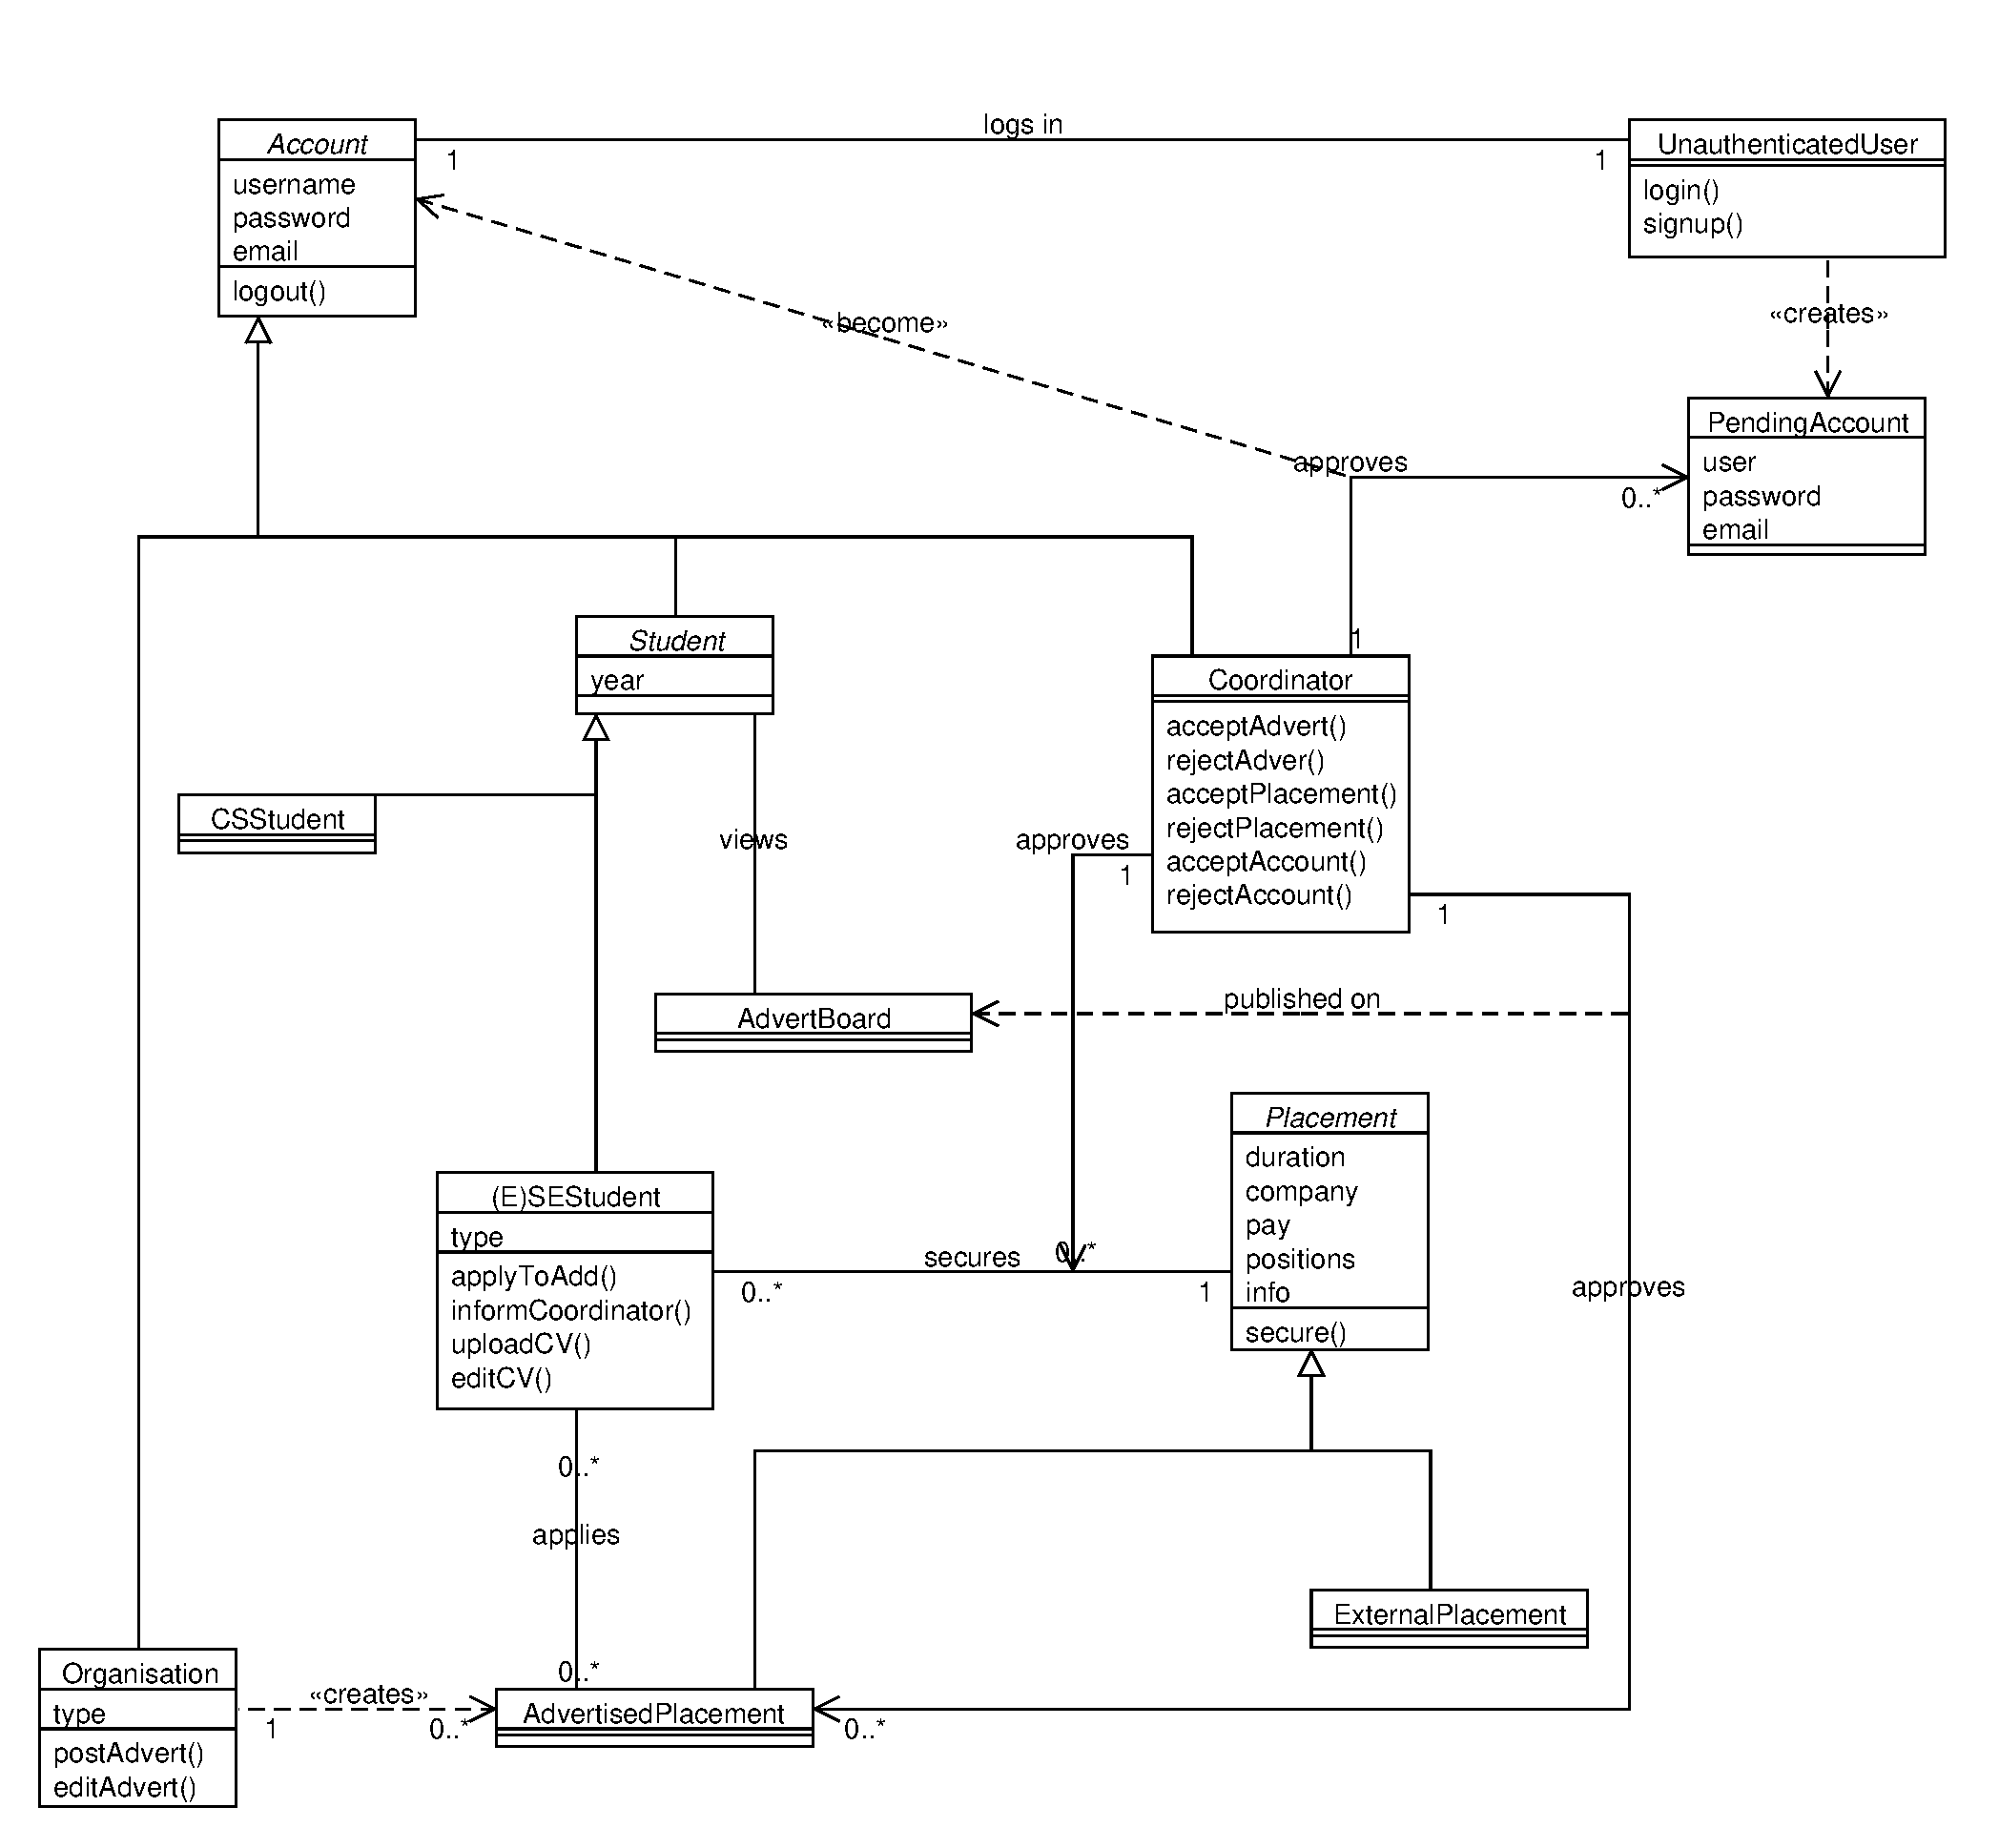
\includegraphics[scale=0.45]{domain_model_v2.pdf}\\
Unauthenticated users represents the guests that visit the system, prior to logging in.\\\
Unauthenticated users can opt to sign up, which creates a PendingAccount instance, that needs to be approved by a Coordinator. Once the Coordinator approves it, the PendingAccount becomes one of the three types of Account, and can then be used for logging in.\\

Account is a generalisation representing user accounts. This branches off to three types of account - Organisation, Coordinator and Student.\\

Organisations represent either Companies or Academics (distinguished by type). They create AdvertisedPlacements that, once approved by a Coordinator, become visible on the AdvertBoard.\\

Students are either ordinary Computing Science students, in which case they can only view adverts, or (Electronic) Software Engineering students, which can also apply to the placements that are visible on the Advert Board.\\

Students can secure placements, either from the ones visible on the AdvertBoard, or from external sources. Coordinators need to approve the securing of placements.


%%%%%%%%%%%%%%%%%%%%%%%%%%%%%%%%%%%%%%%%%%%%%%%%%%%%%%%%%%%%%%%%%%%%%%%%%%%%%%
\newpage
\section{Use Case Descriptions}
This section describes the key features which are required for the system. These can be broken into four categories as follows:\
\begin{itemize}
\item{\textbf{Utilities / Account Management}
	\begin{itemize}
		\item{Login}
		\item{Account creation}
	\end{itemize}}
\item{\textbf{Coordinator Administration}
	\begin{itemize}
		\item{Advert approval}
		\item{Mark placements as filled}
	\end{itemize}}
\item{\textbf{Advert Submission}
	\begin{itemize}
		\item{Submission of adverts by organisations}
		\item{Submission of external placements by students}
	\end{itemize}}
\item{\textbf{Advert viewing and applications}
	\begin{itemize}
		\item{Viewing of adverts}
		\item{Application for placement through system}
		\item{Notification of successfully securing a placement}
	\end{itemize}}
\end{itemize}



\newpage
\subsection{Utilities / Account Management}
Use Case Diagram\\
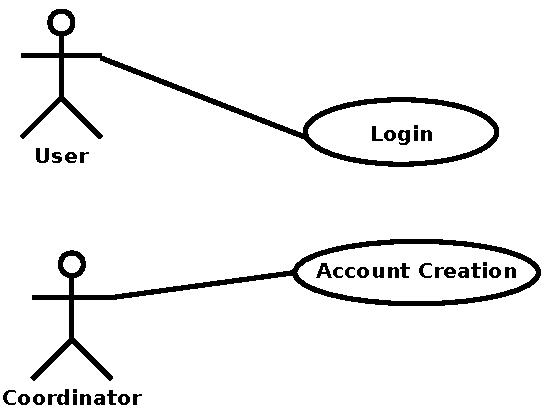
\includegraphics{Utilities.pdf}

\begin{UseCaseTemplate}
\UseCaseLabel{Login}
\UseCaseDescription{
\begin{enumerate}
\item{User enters account name and password into appropriate field.}
\item{User presses enter/confirm.}
\item{IF (details are correct) THEN GOTO 4 ELSE GOTO 5.}
\item{Prompt user reenter details. GOTO 1.}
\item{END}
\end{enumerate}
}
\UseCaseRationale{Identified a need for different classes of user to have a different range of functionality presented. For example only the coordinator should be able to approve adverts. Indentified at client interview.}
\UseCasePriority{Must Have}
\UseCaseStatus{Implemented}
\UseCaseActors{User}
\UseCaseExtensions{}
\UseCaseIncludes{}
\UseCaseConditions{\begin{itemize}
\item{\textbf{pre}\ user must have an account created in the system}
\end{itemize}}
\UseCaseNonFunctionalRequirements{\begin{itemize}
\item{Login should be GUID for students and generated for companies.}
\end{itemize}
}
\UseCaseScenarios{\begin{itemize}
\item{\textbf{Primary:}\ Mark enters his username and password into the corresponding fields and selects login. He is logged into the system successfully.}
\item{\textbf{Alternate 1:}\ Ross makes a typing mistake whilst entering his password and attempts to login. The system reports this error and prompts him to reenter his password.}
\item{\textbf{Alternate 2:}\ Craig wishes to login to the system but has forgotten his details. He chooses to have his password sent to him. He enters his email to which the account is registered and selects send. Using
the details emailed to him he successfully logs in.}
\end{itemize}}
\UseCaseRisks{}
\UseCaseUserInterface{Username/Password input fields}
\end{UseCaseTemplate}


\begin{UseCaseTemplate}
\UseCaseLabel{Account Creation}
\UseCaseDescription{
\begin{enumerate}
\item{User chooses an account type (Organisation or Student) .}
\item{User is prompted for an account username. IF (the account name is taken) THEN prompt the user to enter another name and repeat.}
\item{Prompt user to enter password and then enter it again to confirm. IF (passwords dont match) THEN alert the user and repeat.}
\item{Continue to prompt user for relevant data in this fashion.}
\item{END}
\end{enumerate}
}
\UseCaseRationale{To interact on an individual basis with the system, it must have some way of telling who is using it. Identified in business cases / client interview.}
\UseCasePriority{Must Have}
\UseCaseStatus{Not Implemented}
\UseCaseActors{Coordinator}
\UseCaseExtensions{}
\UseCaseIncludes{}
\UseCaseConditions{\begin{itemize}
\item{\textbf{pre}\ A user exists for whom an account must be created.}
\end{itemize}}
\UseCaseNonFunctionalRequirements{\begin{itemize}
\item{For students their account details should match their GUID login.}
\item{Usernames must be unique.}
\end{itemize}}
\UseCaseScenarios{
\begin{itemize}
\item{\textbf{Primary:}\ Tim wishes to create a new account. He selects an option to create a new account and enters a username and initial password for the user. He then confirms his selection. The system informs him that his choice of username is valid and the account is created. }
\item{\textbf{Alternate 1:}\ Rose attempts to confirm a new account, but the username she has entered is already in use. The system informs her of this and she chooses an alternative username instead. She confirms this new username and the account is successfully created.}
\end{itemize}}
\UseCaseRisks{}
\UseCaseUserInterface{A field based input for each value required}
\end{UseCaseTemplate}




%%%%%%%%%%%%%%%%%%%%%%%%%%%%%%%%%%%%%%%%%%%%%%%%%%%%%%%%%
\newpage
\subsection{Coordinator Administration}
Use Case Diagram\\
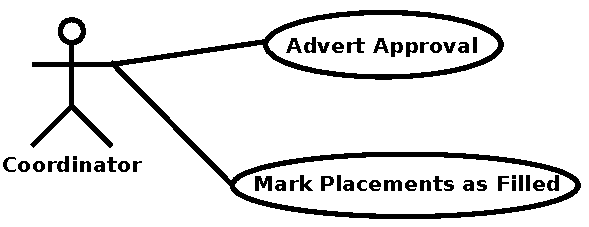
\includegraphics{CoordinatorAdministration.pdf}

\begin{UseCaseTemplate}
\UseCaseLabel{Advert Approval}
\UseCaseDescription{
\begin{enumerate}
\item{User selects an advert.}
\item{User selecnts 'approve' and confirms.}
\item{Advert is made visible to students.}
\item{END}
\end{enumerate}
}
\UseCaseRationale{Course coordinator needs to be able to assess advert to be visible for course coordinator. Identified in business case / client interview.}
\UseCasePriority{Must Have}
\UseCaseStatus{Not Implemented}
\UseCaseActors{Coordinator}
\UseCaseExtensions{Email approved adverts to students}
\UseCaseIncludes{
\begin{itemize}
\item{Login}
\item{Viewing of adverts}
\end{itemize}
}
\UseCaseConditions{\begin{itemize}
\item{\textbf{pre} Advert must exist.}
\item{\textbf{post} Advert is marked as approved and becomes viewable to students.}
\end{itemize}}
\UseCaseNonFunctionalRequirements{Prompt for confirm before approving advert.}
\UseCaseScenarios{\begin{itemize}
\item{\textbf{Primary:}\ John logs in and searches for unapproved adverts on the advert board. He finds one such advert and determines whether the advert is suitable for the course. Then, he marks the advert as approved, confirming his choice when prompted.}
\item{\textbf{Alternate 1:}\ Kate logs in and search for unapproved adverts. Then she accidentally clicks approve advert without determining the purpose of the course carefully. At the confirm prompt, she cancels the approval.}
\end{itemize}}
\UseCaseRisks{Advert may be accidentally approved before editing is complete or when advert is unsuitable. Even with error checking prompts this is still a possibility.}
\UseCaseUserInterface{}
\end{UseCaseTemplate}


\begin{UseCaseTemplate}
\UseCaseLabel{Mark Placements as Filled}
\UseCaseDescription{\begin{enumerate}
\item{User selects an advert}
\item{User chooses to mark the placement as filled and confirms}
\item{Advert now appears as taken in advert board}
\item{END}
\end{enumerate}}
\UseCaseRationale{There is obviously a need to communicate that a placement has been successfully filled so that other students dont waste their time making applications to it. However the client requested that in this situation the advert should not be removed, in case the placement becomes available again. Identified at client interview.}
\UseCasePriority{Should Have}
\UseCaseStatus{Not Implemented}
\UseCaseActors{Coordinator}
\UseCaseExtensions{}
\UseCaseIncludes{Viewing of Adverts}
\UseCaseConditions{\begin{itemize}
\item{\textbf{pre}\ an advert exists for a placement which a student has filled.}
\item{\textbf{post}\ this advert is marked as taken on the advert board.}
\end{itemize}}
\UseCaseNonFunctionalRequirements{Persistence of advert after marking it as filled}
\UseCaseScenarios{
\begin{itemize}
\item{\textbf{Primary:}\ Valerie logs in and has a placement she wishes to mark as fulfilled by a student. She scrolls through the advert board until she finds
the advert, selects in and chooses an option to mark it as taken.}
\item{\textbf{Alternate 1:}\ Margaret logs in and searches the advert board for a placement she wishes to mark as taken. She mistakenly selects the wrong placement and proceed to mark it as taken.
Upon realising her mistake, she reselects the advert and chooses to reopen the advert for submissions.}
\end{itemize}}
\UseCaseRisks{User could mistakenly mark an advert as taken and leave the system, making the advert appear closed to students ( and therfore most likely leave a taken advert
marked as unfulfilled), failing to notice their mistake.}
\UseCaseUserInterface{}
\end{UseCaseTemplate}


%%%%%%%%%%%%%%%%%%%%%%%%%%%%%%%%%%%%%%%%%%%%%%%%%%%%%%%%%%%%%%%%%%%%%%%%%%%%%%%%%%%
\newpage
\subsection{Advert Submission}
Use Case Diagram\\
\\
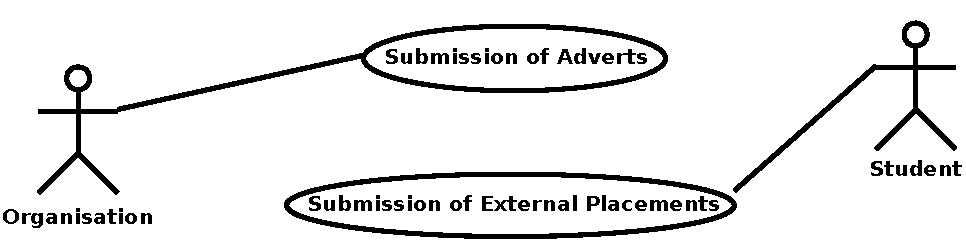
\includegraphics{AdvertSubmission.pdf}


\begin{UseCaseTemplate}
\UseCaseLabel{Submission of Adverts}
\UseCaseDescription{
\begin{enumerate}
\item{User chooses 'submit advert'.}
\item{Prompt for input into advert fields.}
\item{User confirms their input.}
\item{Advert is added to system, pending approval.}
\item{END}
\end{enumerate}
}
\UseCaseRationale{This is a core feature of the system. Identified in the business case}
\UseCasePriority{Must Have}
\UseCaseStatus{Not Implemented}
\UseCaseActors{Organisation}
\UseCaseExtensions{}
\UseCaseIncludes{Login}
\UseCaseConditions{\begin{itemize}
\item{\textbf{pre}\ The organisation must have already obtained a login for the system. The organisation must be logged in.}
\item{\textbf{post}\ The advert is queued to be reviewed by the course coordinator before being visible to the users of the system.}
\end{itemize}}
\UseCaseNonFunctionalRequirements{\begin{itemize}
\item{Normally for the established organisations, a link to the application page of the organisation should be included in the description. Also organisations can post links to more info in the ad.}
\end{itemize}
}
\UseCaseScenarios{
\begin{itemize}
\item{\textbf{Primary:}\ Apple Inc. logs in successfully. They select the ‘Submit Advertisement’ menu item and are taken to the correct page. They fill in all fields and click the ‘Confirm’ button at the bottom of the page. A confirmation is displayed saying that the advert submission was successful.}
\item{\textbf{Alternate 1:} Dr. Jones logs in successfully. He selects the ‘Submit Advertisement’ menu item and is taken to the correct page. He enters details in the fields and clicks ‘Confirm’. An error message is displayed saying that not all fields have been filled out. Dr. Jones fill in the missing fields and clicks ‘Confirm’ again. A confirmation is displayed saying the advert submission was successful.}
\end{itemize}
}
\UseCaseRisks{}
\UseCaseUserInterface{Structure Input Form}
\end{UseCaseTemplate}


\begin{UseCaseTemplate}
\UseCaseLabel{Submission of External Placement}
\UseCaseDescription{\begin{enumerate}
\item{User chooses 'submit advert'.}
\item{Prompt for input into advert fields}
\item{User confirms their input.}
\item{Advert is added to system, pending approval.}
\item{END}
\end{enumerate}}
\UseCaseRationale{A student must get an internship approved by submitting the internship details. Identified at client interview.}
\UseCasePriority{Should Have}
\UseCaseStatus{Not Implemented}
\UseCaseActors{Student}
\UseCaseExtensions{}
\UseCaseIncludes{Login}
\UseCaseConditions{\begin{itemize}
\item{\textbf{pre}\ The student must have already obtained a login for the system (by automatic assignment or from the course coordinator). The student must be logged in.}
\item{\textbf{post}\ The advert is queued to be reviewed by the course coordinator.}
\end{itemize}}
\UseCaseNonFunctionalRequirements{Structured input form}
\UseCaseScenarios{\begin{itemize}
\item{\textbf{Primary:}\ Barry wants to submit an advert to be reviewed. He logs in to the system, clicks the submit advert button under the review section and fills in the details. It gives him a message confirming the success of the operation.}
\end{itemize}
}
\UseCaseRisks{}
\UseCaseUserInterface{}
\end{UseCaseTemplate}



\newpage
\subsection{Advert Viewing and Applications}
Use Case Diagram\\
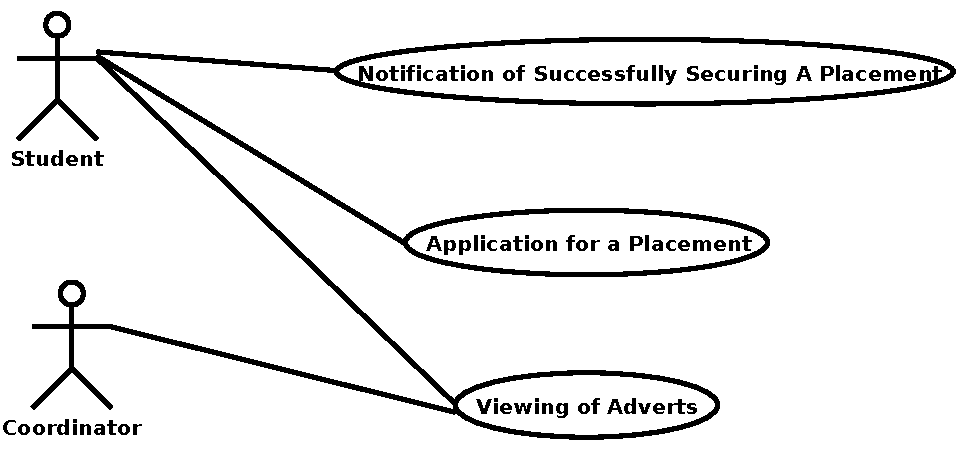
\includegraphics{AdvertViewingAndApplications.pdf}

\begin{UseCaseTemplate}
\UseCaseLabel{Viewing of Adverts}
\UseCaseDescription{
\begin{enumerate}
\item{Adverts are displayed on screen.}
\item{END}
\end{enumerate}
}
\UseCaseRationale{Fundamental to system description. Initial need specified in business case and exact method for viewing adverts elaborated in client interviews}
\UseCasePriority{Must Have}
\UseCaseStatus{Not Implemented}
\UseCaseActors{\begin{itemize}
\item{Organisation}
\item{Student}
\item{Coordinator}
\end{itemize}}
\UseCaseExtensions{}
\UseCaseIncludes{Login}
\UseCaseConditions{None}
\UseCaseNonFunctionalRequirements{}
\UseCaseScenarios{
\begin{itemize}
\item{\textbf{Primary:}\ John logs in and attempts to find a suitable placement on the advert board. He scrolls down through the advert board until he finds a suitable placement, or there are no adverts left to view. He closes the interface.}
\end{itemize}
}
\UseCaseRisks{}
\UseCaseUserInterface{}
\end{UseCaseTemplate}

\begin{UseCaseTemplate}
\UseCaseLabel{Application for Placement}
\UseCaseDescription{\begin{enumerate}
\item{User finds advert they wish to apply for on the advert board}
\item{They select this advert and choose 'Apply'}
\item{Prompt user for relevant info.}
\item{User confirms and sends application.}
\item{END}
\end{enumerate}
}
\UseCaseRationale{Some smaller companies may not have their own application process so in this scenario, the client has expressed a preference for applications to be handled through the system. Current version identified as a result of requirements forum.}
\UseCasePriority{Could Have}
\UseCaseStatus{Not Implemented}
\UseCaseActors{Student}
\UseCaseExtensions{}
\UseCaseIncludes{Viewing of Adverts}
\UseCaseConditions{\begin{itemize}
\item{\textbf{post}\ application has been submitted and made visible to company}
\end{itemize}}
\UseCaseNonFunctionalRequirements{Structured input form}
\UseCaseScenarios{
\begin{itemize}
\item{\textbf{Primary:}\ Karl wishes to submit an application for an advert a friend told him about. He finds the advert on the board and chooses to submit
an application. He enters all relevant extra data and sends off the application. He exits the system.}
\item{\textbf{Alternate 1:} Ian selects an advert and chooses to submit an application. When prompted to enter any extra details he accidentally clicks send. He is prompted to confirm he wishes to submit the application. Thanks to this warning he recovers the error and enters data. He submits the application
}
\end{itemize}
}
\UseCaseRisks{Student could send away incomplete or erroneous applications accidentally. No method exists to retrieve/edit such an application}
\UseCaseUserInterface{}
\end{UseCaseTemplate}

\begin{UseCaseTemplate}
\UseCaseLabel{Notification of Successfully Securing a Placement}
\UseCaseDescription{
\begin{enumerate}
\item{Student selects a placement from the advert board}
\item{They choose to notify that they have secured this placement}
\item{IF (the placement is alread filled) THEN user is notified and submission is ignored. GOTO 2}
\item{Notification is recieved and put into system for confirmation by coordinator}
\item{END}
\end{enumerate}
}
\UseCaseRationale{Course coordinator must ensure that every course student has their work placement.}
\UseCasePriority{Could Have}
\UseCaseStatus{Not Implemented}
\UseCaseActors{Student}
\UseCaseExtensions{}
\UseCaseIncludes{Login}
\UseCaseConditions{\begin{itemize}
\item{\textbf{pre}\ Advert must exist. }
\item{\textbf{pre}\ Advert must be approved by course coordinator.}
\item{\textbf{pre} Organisation has to secure the placement position for student.}
\item{\textbf{post} Course student's status is marked as secure}
\end{itemize}}
\UseCaseNonFunctionalRequirements{}
\UseCaseScenarios{\begin{itemize}
\item{\textbf{Primary:}\ Andrew logs in and look for desirable and approved advert. He clicks on secure the placement button and sends an email about the selected placement to course coordinator.}
\item{\textbf{Alternate 1:}\ Margaret logs in and select desirable advert but she cannot click on secure the placement button because the organisation she applies for has not accepted her position.}
\end{itemize}}
\UseCaseRisks{It may take time for the organisation to secure student's position.}
\UseCaseUserInterface{}
\end{UseCaseTemplate}


%%%%%%%%%%%%%%%%%%%%%%%%%%%%%%%%%%%%%%%%%%%%%%%%%%%%%%%%%%%%%%%%%%%%%%%%%%%%%%
\newpage
\section{Non Functional Requirements}
\begin{itemize}
\item{When the deadline for a placement has been reached, the placement should remain visible for one week after the deadline before being removed from the advert board}
\item{There should be a single interface, but different dashboards available to the user type once the user logs in.}
\item{Getting login details to the company could be done by email -- an email could be sent to the company with registration details and the course coordinator would approve the request for the company to be part of the system.}
\end{itemize}


%%%%%%%%%%%%%%%%%%%%%%%%%%%%%%%%%%%%%%%%%%%%%%%%%%%%%%%%%%%%%%%%%%%%%%%%%%%%%%

\section{Conflicts and Resolution}
\textbf{Conflict}: Originally in client interview it was established that students could be able to make applications through the system directly to companies. However at the stakeholder panel it was suggested that this feature was outside of the system's scope.
\textbf{Resoultion - \date{2012/11/08}}: The question of whether this feature should or should not be implemented was raised by the team in the Requirements Forum. compromise the team chose to keep this feature as a potential use case but relegated it from a must have to a could have status.\\


%%%%%%%%%%%%%%%%%%%%%%%%%%%%%%%%%%%%%%%%%%%%%%%%%%%%%%%%%%%%%%%%%%%%%%%%%%%%%%

\appendix
\section{Change Log}
\subsection{Version 1}
\begin{enumerate}
\setcounter{enumi}{-1}
\item{Inital Draft -- \date{2012/11/01}}
\item{Minor edits / cleanup -- \date{2012/11/09}}
\end{enumerate}

\subsection{Version 2}
\begin{enumerate}
\setcounter{enumi}{-1}
\item{Revision of use cases. Addition of use cases diagrams --  \date{2012/11/11}}
\end{enumerate}
\subsection{Version 3}
\begin{enumerate}
\setcounter{enumi}{-1}
\item{Addition of pseducode descriptions and Conflict and Resolution section -- \date{2012/11/12}}
\end{enumerate}

\section{Glossary}
\textbf{PSD/PSD3}: Professional Software Development 3\\
\textbf{CS}: Computing Science\\
\textbf{SE}: Software Engineering\\
\textbf{ESE}: Electronic Software Engineering\\
\textbf{SESP}: Software Engineering Summer Placement\\
\textbf{GUID}: Glasgow University Identification\\








%%%%%%%%%%%%%%%%%%%%%%%%%%%%%%%%%%%%%%%%%%%%%%%%%%%%%%%%%%%%%%%%%%%%%%%%%%%%%%

\end{document}

%%%%%%%%%%%%%%%%%%%%%%%%%%%%%%%%%%%%%%%%%%%%%%%%%%%%%%%%%%%%%%%%%%%%%%%%%%%%%%
